\documentclass[12pt,article]{article}
\usepackage{lmodern}
\usepackage{amssymb,amsmath}
\usepackage{ifxetex,ifluatex}
\usepackage{fixltx2e} % provides \textsubscript
\ifnum 0\ifxetex 1\fi\ifluatex 1\fi=0 % if pdftex
  \usepackage[T1]{fontenc}
  \usepackage[utf8]{inputenc}
\else % if luatex or xelatex
  \ifxetex
    \usepackage{mathspec}
    \usepackage{xltxtra,xunicode}
  \else
    \usepackage{fontspec}
  \fi
  \defaultfontfeatures{Mapping=tex-text,Scale=MatchLowercase}
  \newcommand{\euro}{€}
\fi
% use upquote if available, for straight quotes in verbatim environments
\IfFileExists{upquote.sty}{\usepackage{upquote}}{}
% use microtype if available
\IfFileExists{microtype.sty}{%
\usepackage{microtype}
\UseMicrotypeSet[protrusion]{basicmath} % disable protrusion for tt fonts
}{}
\usepackage[margin=1in]{geometry}
\ifxetex
  \usepackage[setpagesize=false, % page size defined by xetex
              unicode=false, % unicode breaks when used with xetex
              xetex]{hyperref}
\else
  \usepackage[unicode=true]{hyperref}
\fi
\hypersetup{breaklinks=true,
            bookmarks=true,
            pdfauthor={Justin Murphy and Daniel Devine},
            pdftitle={Does Public Support for UKIP Drive Media Coverage or Does Media Coverage Drive Support for UKIP?},
            colorlinks=true,
            citecolor=blue,
            urlcolor=blue,
            linkcolor=blue,
            pdfborder={0 0 0}}
\urlstyle{same}  % don't use monospace font for urls
\usepackage{graphicx,grffile}
\makeatletter
\def\maxwidth{\ifdim\Gin@nat@width>\linewidth\linewidth\else\Gin@nat@width\fi}
\def\maxheight{\ifdim\Gin@nat@height>\textheight\textheight\else\Gin@nat@height\fi}
\makeatother
% Scale images if necessary, so that they will not overflow the page
% margins by default, and it is still possible to overwrite the defaults
% using explicit options in \includegraphics[width, height, ...]{}
\setkeys{Gin}{width=\maxwidth,height=\maxheight,keepaspectratio}
\setlength{\parindent}{0pt}
\setlength{\parskip}{6pt plus 2pt minus 1pt}
\setlength{\emergencystretch}{3em}  % prevent overfull lines
\providecommand{\tightlist}{%
  \setlength{\itemsep}{0pt}\setlength{\parskip}{0pt}}
\setcounter{secnumdepth}{0}

%%% Use protect on footnotes to avoid problems with footnotes in titles
\let\rmarkdownfootnote\footnote%
\def\footnote{\protect\rmarkdownfootnote}

%%% Change title format to be more compact
\usepackage{titling}

% Create subtitle command for use in maketitle
\newcommand{\subtitle}[1]{
  \posttitle{
    \begin{center}\large#1\end{center}
    }
}

\setlength{\droptitle}{-2em}
  \title{Does Public Support for UKIP Drive Media Coverage or Does Media Coverage
Drive Support for UKIP?}
  \pretitle{\vspace{\droptitle}\centering\huge}
  \posttitle{\par}
  \author{Justin Murphy and Daniel Devine}
  \preauthor{\centering\large\emph}
  \postauthor{\par}
  \date{}
  \predate{}\postdate{}

\usepackage{dcolumn}
\usepackage{setspace}

% Redefines (sub)paragraphs to behave more like sections
\ifx\paragraph\undefined\else
\let\oldparagraph\paragraph
\renewcommand{\paragraph}[1]{\oldparagraph{#1}\mbox{}}
\fi
\ifx\subparagraph\undefined\else
\let\oldsubparagraph\subparagraph
\renewcommand{\subparagraph}[1]{\oldsubparagraph{#1}\mbox{}}
\fi

\begin{document}
\maketitle

\begin{abstract}
Previous research suggests media attention may cause support for populist right-wing parties, but this finding is debated and extant evidence remains limited to proportional representation systems in which such an effect would be most likely. At the same time, in the United Kingdom's first-past-the-post system, an ongoing political and regulatory debate revolves around whether the media give disproportionate coverage to the populist right-wing UK Independence Party (UKIP). Thus, we use a mixed-methods approach to investigate the causal dynamics of UKIP support and media coverage as an especially valuable case. Vector autoregression (VAR) using monthly, aggregate time-series data from 2004 to September 2015 provides new evidence consistent with a model in which media coverage drives party support, but party support does not drive media coverage. Additionally, qualitative investigation of the dynamics suggests that in at least two key periods of stagnating or declining support for UKIP, media coverage increased and was followed by increases in public support. Overall the findings show that media coverage can and does appear to drive public support in a substantively important fashion irreducible to previous levels of public support, even in a national institutional environment least supportive of such an effect. The findings have direct and troubling implications for contemporary political and regulatory debates in the United Kingdom and potentially liberal democracies more generally.
\end{abstract}
\doublespacing

\section{Introduction}\label{introduction}

If the visibility of a political party in the media shapes the public
support it receives, then the degree to which the media gives attention
to different political parties can have significant implications for
democracy. In the United Kingdom, critics allege that the media pays
disproportionate attention to the populist, right-wing UK Independence
Party (UKIP) but media elites claim that media coverage of UKIP is
driven by increasing public support for the party. Descriptively, media
attention to UKIP is greater than that given to other, similarly sized
parties on the right as well as the left (Goodwin and Ford, 2013;
Stevenson, 2014; Soussi, 2014), but UK media regulator Ofcom as well as
the BBC have publicly defended the attention paid to UKIP on grounds of
public support for the party (Sweeney, 2015; Wintour, 2015). Implied in
this elite reasoning is a causal model, namely that public support
drives media coverage rather than vice-versa.

Yet previous research from proportional representation systems suggests
that public support does not drive media coverage for populist
right-wing parties, but rather their media coverage drives their public
support (Boomgaarden and Vliegenthart, 2007, 2009; Vliegenthart et al.,
2012). By leveraging this insight to investigate the causal dynamics of
UKIP support and media coverage, we fill an important gap in current
research on the visibility-support nexus and contribute pragmatically
relevant insights to a contentious public policy debate of broad social
significance (Gerring, 2015). First, we contribute to current research
on the visibility-support nexus by testing a key insight from this
research in a new institutional context where hypothesized relationship
should be less likely. Because proportional representation systems are
associated with a greater number of small parties (Duverger, 1972) and
they tend to produce more diverse news (Benson, 2009; Sheafer and
Wolfsfeld, 2009; Kumlin, 2001; Strömbäck and Dimitrova, 2006; Baum,
2012), research confined to such systems is arguably most likely to
reflect a model in which media coverage generates support for populist
right-wing parties. In a first-past-the-post system, where we typically
expect only two parties and media to be less diverse, these
institutional pressures make it more difficult for the media to generate
support for smaller populist, right-wing parties. Thus, testing this
theory with time-series data from a first-past-the-post system
contributes to either refining the scope conditions of previous research
(in the case of unexpected findings) or else extending and strengthening
our confidence in the media-support relationship. Additionally, we
contribute to a pressing regulatory question in UK national politics, as
the democratic quality of UK media regulation with respect to political
party favouritism, especially regarding populist right-wing parties,
remains on public trial. This article lends insight into the causal
dynamics implied but rarely if ever tested within such popular policy
debates.

The article begins by outlining the theory from which we are generating
our expectations, and outlines our hypotheses. It then moves on to a
discussion on the data, method and research strategy we use to
investigate these hypotheses, before discussing the findings and
implications. We then present a qualitative analysis of the growth of
UKIP to support the quantitative findings, before concluding.

\section{Theory}\label{theory}

A large body of research suggests that mass media coverage, as the
primary channel through which the electorate receives information about
politicians and parties, affects many different aspects of electoral
politics (Norris, 2000; Paletz, 1996; Beck et al., 2002; Dalton et al.,
1998). If media coverage of political parties is driven by public
support for the parties--even if media coverage then increases public
support further--it could be argued that media are facilitating popular
sovereignty. On the other hand, if media coverage independently changes
public support rather than reflects it, this would represent a point of
crucial possible distortion in the functioning of a democracy. The
latent normative motivation for the present investigation is whether the
quantity of UKIP's media coverage represents a form of media bias which
generates rather than reflects public opinion, or if the media's
fascination with UKIP is a democratically appropriate effect of public
opinion.

One current of previous research on the dynamics of media coverage and
party support finds evidence consistent with the argument that the
quantity of media coverage given to a political party drives public
support for that party. Walgrave and De Swert (2004) find that, in
time-series data from Belgium, the evidence reflects a model in which
newspapers and television stations helped to increase the electoral
results of the Vlaams Blok by emphasising political issues owned by the
extreme right-wing party. Boomgaarden and Vliegenthart (2007;
Vliegenthart and Boomgaarden, 2010) find that in the Netherlands,
quantity of media coverage on immigration-related topics is associated
with a subsequent increase in the vote-share for anti-immigrant parties,
controlling for objective factors such as levels of immigration.
Boomgaarden and Vliegenthart (2009) also find, using time-series from
Germany, that media coverage of immigrant actors is associated with
subsequent change in public attitudes toward immigration, conditional on
objective factors such as immigration levels. While much of the previous
research above considers the political implications of issue coverage in
the media, Vliegenhart, Boomgaarden, and Van Spanje (2012) advance this
current further by analyzing time-series on the coverage of parties and
public support for anti-immigrant parties per se in Belgium,
Netherlands, and Germany. That study finds evidence suggesting that
party and party leader visibility is associated with the electoral
outcomes of the parties, but not vice-versa. In another study, media
coverage was found to be one of the best predictors of electoral success
in the 2007 Dutch election (Hopmann et al., 2010). Finally, it has been
shown that in the Netherlands, media coverage of Fortuyn appears to have
improved polling performance of the party before the 2002 election
(Koopmans and Muis, 2009).

Considering research at the individual level, panel data from the
Netherlands suggests that media coverage drives perceptions of
right-wing populist politicians as well as mainstream politicians (Bos
et al., 2011). Media coverage has also been found to help explain
individual-level party preferences in Germany (Semetko and Schoenbach,
1994) and the Netherlands (Oegema and Kleinnijenhuis, 2009). Based on
this previous research, we test the following hypothesis.

H1: Increases in media coverage lead to increased public support,
controlling for previous levels of public support and previous levels of
media coverage.

It is also theoretically plausible, as some scholars have argued, that
changes in party support lead to changes in media coverage (Pauwels,
2010). As Vliegenthart and Boomgaarden (2010) consider, quantity of
media coverage may be driven by the power and position of political
figures. This pattern has been observed, in some cases, in America
(Sellers and Schaffner, 2007) and Switzerland (Tresch, 2009). Sellers
(2007) finds that the types of events U.S. Senators hold, and the guests
of those events, affects the number of news stories written. Tresch
(2009) finds that the amount of coverage given to Swiss legislators is
most importantly a function of leadership and authority criteria related
to the individual politicians. Although both of these studies focus on
politicians rather than political parties per se, they suggest that
variable aspects of political entities have predictable effects on media
visibility. In a study on the diffusion of populist discourse in the
media, Rooduijn (2014) argues from a study of five Western European
countries (Italy, France, Germany, Netherlands, and United Kingdom) the
electoral success of populist parties affects the degree of populism in
the
media.\footnote{Interestingly, in the study by Rooduijn, UKIP is classified as the least successful case of a populist party, based on their electoral results as of 2005, yet populism in British newspapers in 2005 is near that found in Netherlands and Germany and greater than that found in France. Although the findings are interpreted as electoral politics driving media content, Rooduijn's data show that in the UK at least, populism in the media was comparatively high in cross-national perspective before UKIP rose to its recent prominence.}

In line with this current of research, British media and media
regulators have publicly argued media coverage given to political
parties is based on public support for the parties. In its draft
electoral guidelines published in January 2015, the BBC classified UKIP
as deserving a degree of coverage comparable to the ``larger parties,''
because they ``demonstrated a substantial increase in electoral
support,'' as measured by electoral and polling results, between 2010
and 2015 (Sweeney, 2015; BBC, 2015). Ofcom, the UK broadcast regulator,
also included UKIP as a ``major party'' for the purposes of the 2015
General Election and local elections in England and Wales (Ofcom, 2015),
also explicitly on the grounds of improving electoral and polling
results since 2010 (Wintour, 2015). Based on this current of previous
research and the stated reasoning of elite entities with uniquely strong
influence on media agendas, we propose the following additional
hypothesis opposite to H1.

H2: Increases in public support for UKIP lead to increased media
coverage, controlling for previous levels of media coverage and previous
levels of public support.

The following section discusses the data and method we pursue to test
these two hypotheses.

\section{Data, Method, and Research
Strategy}\label{data-method-and-research-strategy}

To measure public support for UKIP, we gathered monthly aggregate
polling data on vote intentions from Ipsos MORI (Ipsos-MORI, n.d.).
Specifically, we constructed the variable \emph{Support} from the
percentage of respondents reporting an intention to vote for UKIP
according to the Ipsos MORI polling for each month. For most months,
this was straightforward because the Ipsos MORI poll is approximately
monthly. For months with multiple polls, we used the poll closest to the
middle of the
month.\footnote{A drawback of this choice is that some polling information is lost, as some polls were not integrated into the dataset. An alternative would be to average all the polls for each month, but this would lead each monthly average to reflect different parts of each month (for instance, if one month has two polls only in the first half, and another month has two polls only in the second half). Because our main interest relates to dynamics, it seems more important to have consistent measures reflecting as close as possible the middle of each month, at the cost of some information loss, than to include more polls but inconsistently reflect different parts of each month.}
For the very few months with no poll or a poll at the border between the
previous or following month, the value was counted as missing and then
all missing values were linearly interpolated. To measure media coverage
of UKIP, we gathered monthly counts of all UK national newspaper reports
mentioning either ``UKIP'' or ``UK Independence Party'' from the
database
Nexis.\footnote{Duplicate articles defined by Nexis's definition of high similarity were excluded.}
The variable \emph{Articles} reflects the number of articles Nexis
returns from the first day of each month until the last day of each
month. Figure 1 provides a summary view of the two main variables of
interest. The dotted line represents \emph{Support} and the solid line
represents \emph{Articles}. Raw values are displayed in the first two
(top) panels. For ease of direct comparison the bottom panel displays
standardized scores in which each value is derived by subtracting the
mean of the particular time-series and dividing by one standard
devation.

It is also plausible that elections have an independent effect on
coverage and support due to general increased media attention and
campaigning. For this reason, we have included eponymous dummy variables
for the months of each national and European election within the
sampling period. The elections included are three European elections
(June 2004, June 2009 and May 2014) and three general elections (May
2005, May 2010, and May 2015). European elections coincide with local
elections in the UK.

In the present analysis we do not consider public opinion on particular
political issues, measures of objective political or policy dynamics, or
the visibility of party leaders in the media, for several reasons. The
first and main reason is dictated by our problem-driven approach.
Because our contribution to the literature is motivated by a particular
debate in the politics of British media, we focus on the parameters of
that debate, which have revolved around party coverage. Although UKIP's
controversial leader Nigel Farage is likely a significant aspect of
UKIP's media visibility, coverage of Farage is almost certainly highly
correlated with coverage of the party, as Vliegenhart, Boomgaarden, and
Van Spanje find of party and leader coverage in multiple other Western
European countries. Second, Vliegenhart, Boomgaarden, and Van Spanje
also find that media coverage of parties is, overall, more relevant than
party leader as a predictor of party support (Vliegenthart et al., 2012:
333). While it is possible that phenomena such as objective immigration
levels, media coverage of immigration, and/or public opinion on
immigration may affect both UKIP party coverage and public support for
UKIP, it is not theoretically straightforward that they should affect
one of our main variables more, or sooner, than the other. Because we
lack any particular theoretical perspective on such possibilities, and
there are many additional causal factors which could arguably be
included in this system, we refrain from proliferating additional
variables (Achen, 2006).

We first use econometric techniques to test for, and distinguish the
ordering of, potential causal dynamics between media coverage and public
support for UKIP. An ideal approach to testing the presented hypotheses
is vector autoregression (VAR) with Granger causality tests (Brandt and
Williams, 2007; Vliegenthart et al., 2012). Specifically, we estimate a
VAR by OLS per equation, using the following form:

\begin{equation}
 \label{eq:VAR}
    y_t = A_1 y_{t-1} + … + A_p y_{t-p} + D_t + u_t
\end{equation}

where \(y_t\) is a \(K \times 1\) vector of endogenous variables and
\(u_t\) is the error term. In our case the endogenous variables are
\emph{Support} and \emph{Articles}. The coefficient matrices \(A_1\),
\ldots{}, \(A_p\) are of dimension \(K \times K\). By convention \(p\)
denotes the ``order'' of the VAR, or the number of lags used. Typically
this is determined empirically, as we do below. In addition, \(D_t\)
refers to a vector of exogenous regressors. In our case the exogenous
regressors include a constant term, a trend term, the dummy variable for
UK General Election months, and the dummy variable of European election
months. We then use the conventional F-type Granger-causality test for
each of the two endogenous variables in the system. The vector of
endogenous variables \(y_t\) is divided into two vectors \(y_1t\) and
\(y_2t\) of dimensionality (\(K_1 \times 1\)) and (\(K_2 \times 1\))
with \(K = K_1 + K_2\) (CITE VAR PACKAGE). The null hypothesis is that
no lags of variable \(y_{1t}\) are significant in the equation for
variable \({y}_{2t}\). If \(α_{21, i} = 0\) for \(i = 1\), \(2\),
\ldots{}, \(p\), we say that \(y_{1t}\) does not ``Granger-cause''
\(y_{2t}\).

Additionally, a brief qualitative historical analysis of the dynamics is
conducted to further probe any potential causal process(es). In
particular, the substantive nature of the puzzle at hand requires the
identification of a causal narrative. Even with econometric evidence
suggesting an association in one direction or the other, it would remain
unclear whether the historical unfolding of such dynamics may imply a
substantively significant issue for the core democratic function under
consideration. In other words, we are not only interested in whether
media coverage amplifies exogenous increases in support--this would be
an important but not necessarily problematic finding from a democratic
perspective. In particular we will have to assess the degree to which
increases in media coverage could possibly generate support for UKIP
\emph{despite low, stagnant, or decreasing} levels of support, in a
historically observable and non-trivial fashion. We explore this
substantive question with a brief but detailed narrative of the
real-world events which coincide behind the time-series plotted in
Figure 1.

\pagebreak

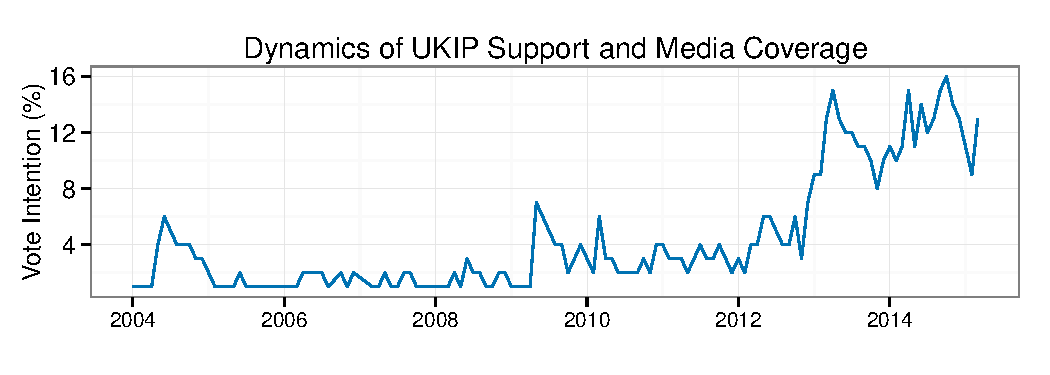
\includegraphics{ukip_media_files/figure-latex/unnamed-chunk-1-1.pdf}
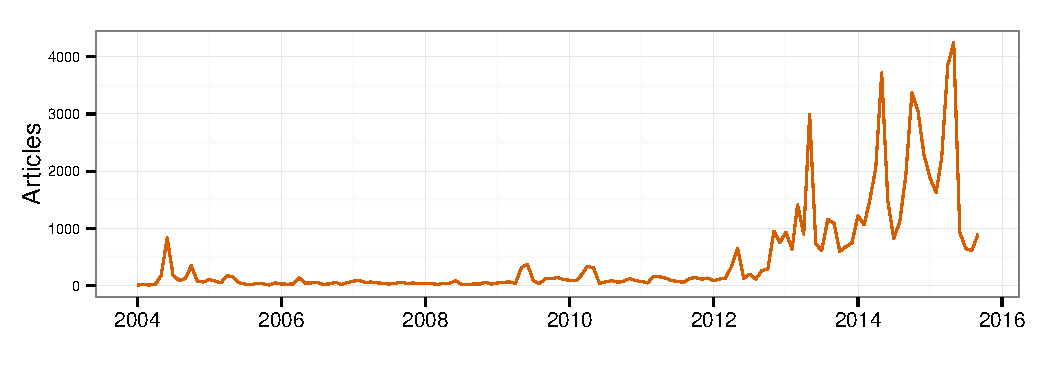
\includegraphics{ukip_media_files/figure-latex/unnamed-chunk-1-2.pdf}

\begin{figure}[htbp]
\centering
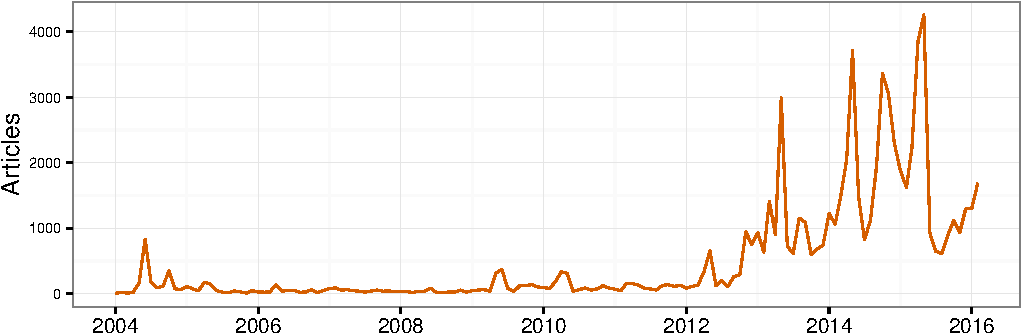
\includegraphics{ukip_media_files/figure-latex/unnamed-chunk-2-1.pdf}
\caption{Dynamics of UKIP Support and Media Coverage}
\end{figure}

\section{Findings and Discussion}\label{findings-and-discussion}

Because both variables are non-stationary, vector autoregression is
estimated with first differences of each variable. Optimal lag length is
determined by the Aikeke Information Criterion to be VAR(3). The model
includes a constant and a trend term. Diagnostics suggest that using the
log of each variable before differencing reduces heteroskedasticity and
serial correlation of errors. Because VAR models have many paramaters to
begin with, monthly indicators controlling for seasonality absorb
crucial degrees of freedom and so are excluded in the intitial models
but added in subsequent models. The models displayed here all pass the
standard ARCH-LM and Portmanteau tests for non-constant error variance
and serial correlation of errors, respectively. Finally, diagnostics
show no evidence of significant temporal instability (see Supplementary
Information).

Surprisingly, initial VAR results show little evidence that changes in
public support predict media coverage, but significant evidence that
media coverage drives public support. As the numerical results and the
Impulse Response plots show, there is no statistically discernable
correlation between past changes in public support and changes in media
coverage, whereas past changes in media coverage have a statistically
significant correlation with changes in public support. Granger
causality tests support this interpretation, with only the latter
relationship nearing conventional cutoffs of statistical significance
(p\textless{}.08).

After including monthly indicators, however, the results reverse: while
the coefficients reflecting the correlation between past changes in
media coverage and public support do not change noticeably, they lose
statistical significance, whereas the coefficients for the other model
become significant and pass the test for Granger causality. Because the
coefficients reflecting the correlation between past changes in media
coverage and public support remain signed as predicted, the increased
standard errors do not necessarily reflect the absence of a relationship
but possibly only a lack of degrees of freedom due to the introduction
of the seasonality indicators.

Additionally, there are limitations of the data which may make it
difficult to identify causal effects in a VAR approach. First, it is
possible that monthly measures are too infrequent to capture causal
effects if the real lag between effects is more shorter than one month.
Importantly, structural tests on all models suggest strong evidence of
instantaneous causality.

Taken together, VAR results suggest qualified evidence for both
directions of causality. While the results are sensitive to the
specification, the results are consistent with the possibility that both
variables drive each other, but that highly robust evidence of this in
one model is not possible due to the nature of the data and the
high-paramater demands of the VAR approach. \pagebreak

\begin{table}[!htbp] \centering 
  \caption{} 
  \label{} 
\begin{tabular}{@{\extracolsep{5pt}}lcc} 
\\[-1.8ex]\hline 
\hline \\[-1.8ex] 
 & \multicolumn{2}{c}{\textit{Dependent variable:}} \\ 
\cline{2-3} 
\\[-1.8ex] & \multicolumn{2}{c}{} \\ 
 & Vote & Articles \\ 
\\[-1.8ex] & (1) & (2)\\ 
\hline \\[-1.8ex] 
 UKIP.Articles.l1 & 0.201$^{*}$ & $-$0.305$^{***}$ \\ 
  & (0.106) & (0.096) \\ 
  & & \\ 
 UKIP.Vote.l1 & $-$0.442$^{***}$ & 0.023 \\ 
  & (0.098) & (0.089) \\ 
  & & \\ 
 UKIP.Articles.l2 & 0.185$^{**}$ & $-$0.257$^{***}$ \\ 
  & (0.093) & (0.085) \\ 
  & & \\ 
 UKIP.Vote.l2 & $-$0.253$^{**}$ & $-$0.083 \\ 
  & (0.102) & (0.092) \\ 
  & & \\ 
 UKIP.Articles.l3 & 0.183$^{**}$ & $-$0.107 \\ 
  & (0.092) & (0.084) \\ 
  & & \\ 
 UKIP.Vote.l3 & $-$0.089 & $-$0.062 \\ 
  & (0.095) & (0.086) \\ 
  & & \\ 
 const & 0.019 & 0.041 \\ 
  & (0.079) & (0.072) \\ 
  & & \\ 
 trend & $-$0.00003 & $-$0.0002 \\ 
  & (0.001) & (0.001) \\ 
  & & \\ 
 General.Elections & 0.111$^{*}$ & 0.336$^{***}$ \\ 
  & (0.060) & (0.055) \\ 
  & & \\ 
 EU.Elections & 0.016 & 0.092 \\ 
  & (0.068) & (0.061) \\ 
  & & \\ 
\hline \\[-1.8ex] 
Observations & 137 & 137 \\ 
R$^{2}$ & 0.153 & 0.368 \\ 
Adjusted R$^{2}$ & 0.093 & 0.323 \\ 
Residual Std. Error (df = 127) & 0.444 & 0.402 \\ 
F Statistic (df = 9; 127) & 2.546$^{**}$ & 8.208$^{***}$ \\ 
\hline 
\hline \\[-1.8ex] 
\textit{Note:}  & \multicolumn{2}{r}{$^{*}$p$<$0.1; $^{**}$p$<$0.05; $^{***}$p$<$0.01} \\ 
\end{tabular} 
\end{table}

\% Table created by stargazer v.5.2 by Marek Hlavac, Harvard University.
E-mail: hlavac at fas.harvard.edu \% Date and time: Tue, Feb 23, 2016 -
16:30:41

\begin{table}[!htbp] \centering 
  \caption{Granger Causality Tests} 
  \label{} 
\begin{tabular}{@{\extracolsep{5pt}} ccc} 
\\[-1.8ex]\hline \\[-1.8ex] 
 & Support & Articles \\ 
\hline \\[-1.8ex] 
P-value & $0.037$ & $0.731$ \\ 
DF1 & $3$ & $3$ \\ 
DF2 & $254$ & $254$ \\ 
F-test & $2.861$ & $0.431$ \\ 
\hline \\[-1.8ex] 
\end{tabular} 
\end{table}

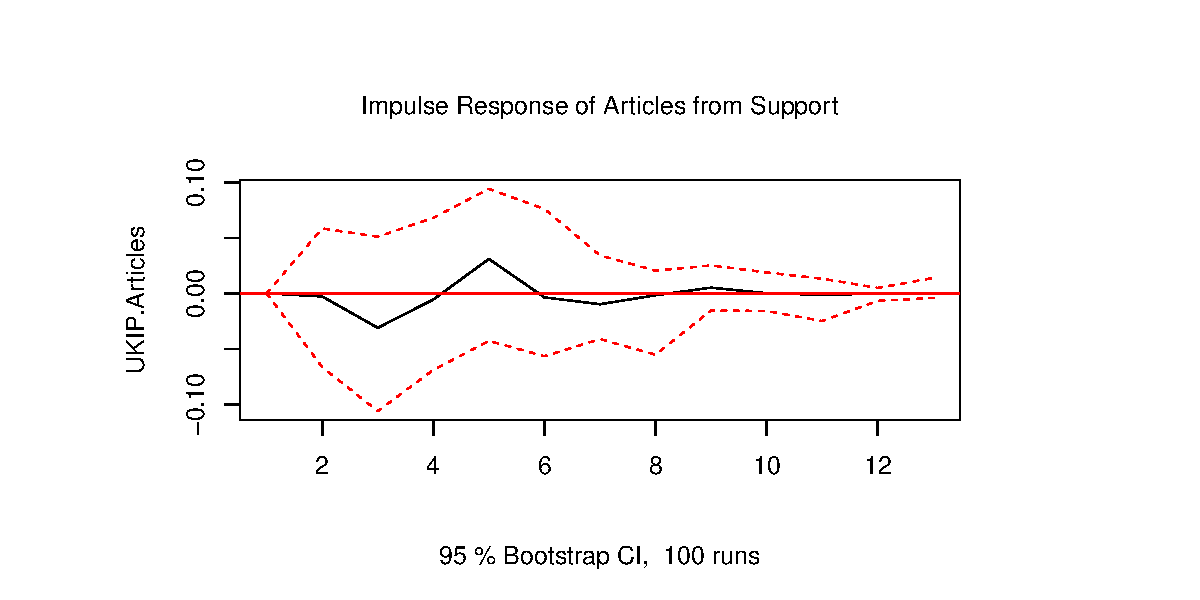
\includegraphics{ukip_media_files/figure-latex/unnamed-chunk-6-1.pdf}
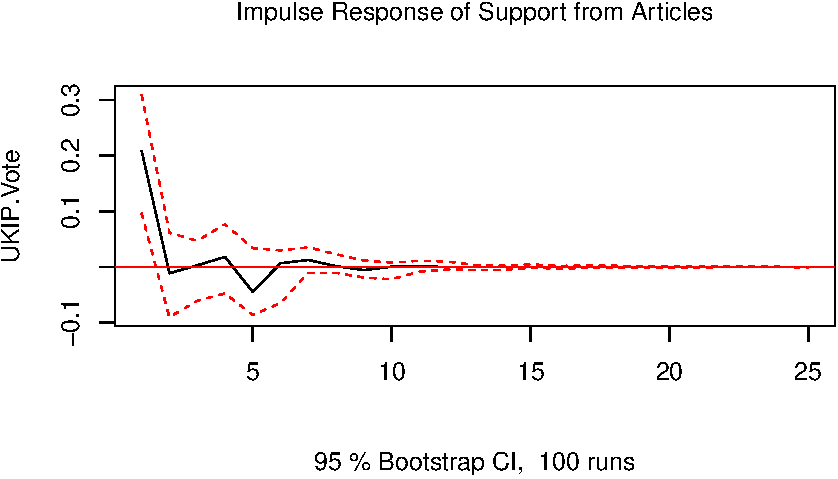
\includegraphics{ukip_media_files/figure-latex/unnamed-chunk-6-2.pdf}

\section{Qualitative Analysis}\label{qualitative-analysis}

UKIP, formed in 1993, began fielding European parliamentary candidates
in 1994 and British parliamentary candidates in 1997. Since then, the
party has enjoyed increasing electoral success, particularly in the
European parliament where the party was the largest in the 2014
election. Until the 2015 general election, UKIP's domestic electoral
success had been much less impressive, receiving just 3.1\% of the vote
in 2010. Like other small or new parties, it has a history of
infighting, changes of direction and leadership, and problems with
financial mismanagement (Whitaker and Lynch, 2011). As recently as 2011,
a lack of media attention was cited as a factor in UKIP's poor
performance, as well as credibility and few activists (Ford et al.,
2012). Indeed, the historical pattern of both media coverage and voting
intention has been one of short spikes followed by a usually drastic
return to low baseline levels (Murphy, 2015).

The party experienced its first bump in both coverage and voting
intention in 2004 with the European election, in which they received
16\% of the vote, where coverage reached 829 articles in a single month,
the highest to date and the highest the party would experience until
2012. During this spike, both media coverage and voting intention
increase proportionately and as would be expected if coverage was driven
by public opinion. Following this, the party experiences a slow decline
in both coverage and support. Over the next eight years, there are a
range of events which attract neither much media attention nor public
support; indeed, similar events occur between these years to those that
occur in later years but which generate much more media attention. The
vast majority of coverage is either in passing, such as election
results, or negative, such as claims of fraud and infighting.

Apart from the 2005 election, in which UKIP received little coverage and
performed very poorly (Anon., 2005; Morris, 2005), UKIP disappeared into
the wilderness until the European elections of 2009. There is a small
boost in both support and coverage in April 2006, when David Cameron
calls the party `fruitcakes, loonies' and `closet racists' (White and
Watt, 2006). Interestingly, this rise in media coverage was followed by
a small but sustained boost in public support, which persisted for three
months. In April 2008, a Conservative MP, Bob Spink, defected, giving
UKIP their first MP which generated very little coverage, despite being
called a coup (Winnett and Prince, 2008). Even the European election in
2009, in which UKIP came second, generated far less coverage than the
2005 European election, where the party came third. Despite this, it was
still hailed as a `political earthquake' (Watt and Taylor, 2009) and
garnered coverage for UKIP's leader Nigel Farage.

\begin{figure}[htbp]
\centering
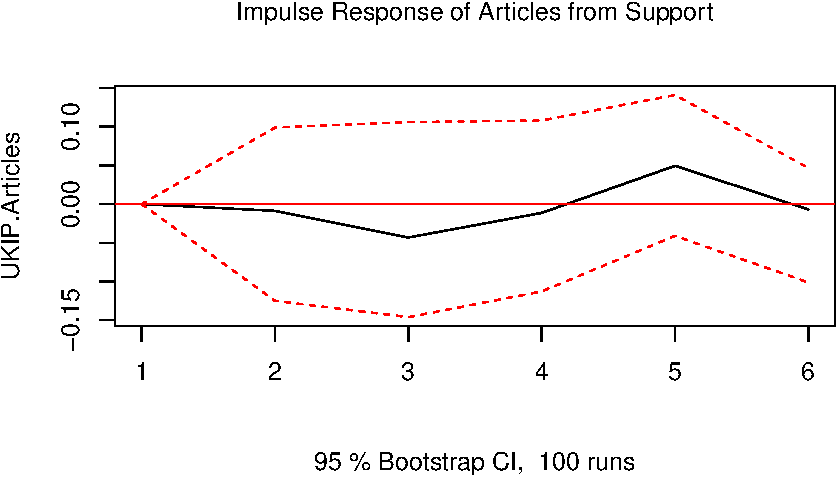
\includegraphics{ukip_media_files/figure-latex/unnamed-chunk-7-1.pdf}
\caption{Standardized Time-Series, Green Lines Indicate Bias and Grey
Lines Indicate Exogenous Increases in Support}
\end{figure}

\begin{figure}[htbp]
\centering
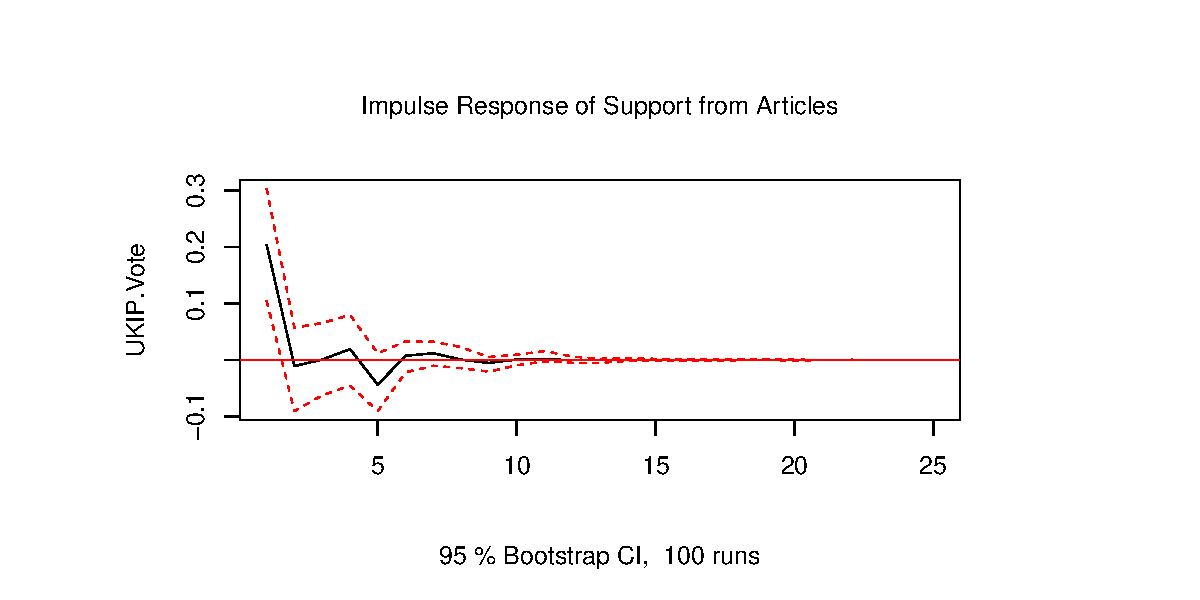
\includegraphics{ukip_media_files/figure-latex/unnamed-chunk-8-1.pdf}
\caption{Standardized Series May 2012 to January 2014}
\end{figure}

\begin{figure}[htbp]
\centering
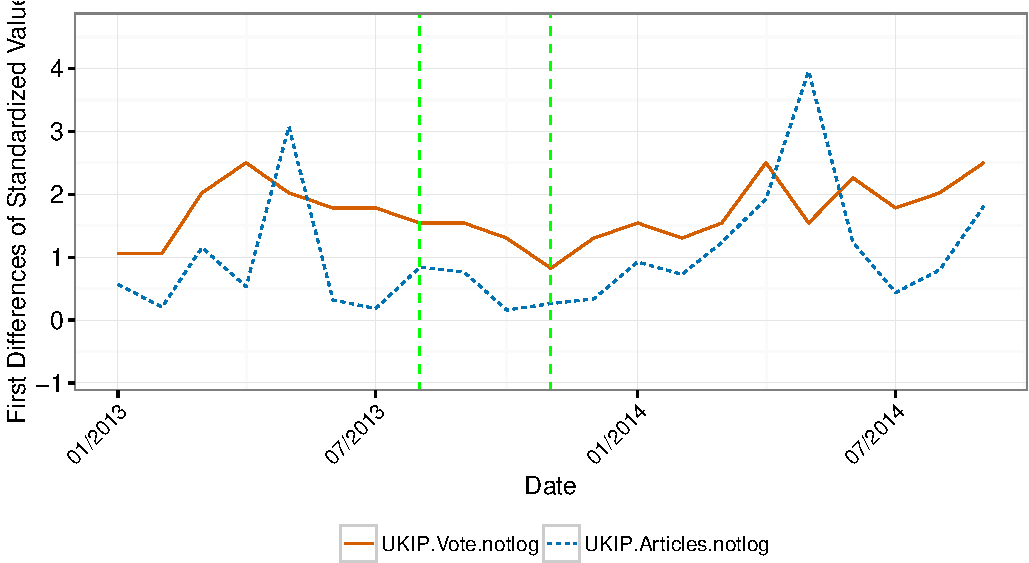
\includegraphics{ukip_media_files/figure-latex/unnamed-chunk-9-1.pdf}
\caption{First Differences of Standardized Series, January 2013 to
September 2014}
\end{figure}

Following this, there are at least two occasions where media coverage
both precludes and seems unrelated to UKIP's performance in opinion
polls, which may then have generated further increases in popular
support (Murphy, 2015). The first occurred between August and November
2012 when, at a point when UKIP's support continued to be unremarkable
and followed a similar pattern as before, the amount of articles
covering UKIP increased from 198 to 948 - the most they have ever
received in one month. This process began with a by-election in Corby,
followed by the UKIP party conference and a controversial Rotherham
by-election (Wainwright, 2012). The media coverage remains consistent
despite unremarkable poll ratings until January 2013, when support for
UKIP spikes and continues on an upward trajectory.

This boost in support continues until May 2013 - a time of local
elections - before beginning to decline, slowly and consistently, from a
high of 15\% in April to 8\% in November 2013: historically quite high,
but not especially so. The second instance is from November 2013 to
December 2014. Despite poll ratings being at their lowest for the entire
year, media coverage begins to increase. It is only following this
perhaps unwarranted coverage that UKIP's poll ratings begin to recover,
and both continue on an upward trajectory through to the end of 2014.
Unlike the previous increase in media coverage, where exogenous events
such as by-elections and conference season were present, it is difficult
to identify a particular incident which was behind the sudden increase
in coverage. One potential mechanism was the lifting of work
restrictions on Romanian and Bulgarian nationals (Martin, 2013) which
occurred in January 2014, with coverage intensifying in the months
before. Whilst this was not directly related to UKIP, the increased
salience of the issues of immigration and the European Union may have
driven the media coverage independent of UKIP's support. Considerable
coverage also surrounded Farage's comments in December 2013 that Britain
should accept Syrian refugees (Goodman, 2013). This may have had the
effect of not just generating coverage but also making UKIP appear a
kinder or more acceptable alternative to the Conservatives.

Previous studies have relied on statistical models similar to the one we
have presented here. However, this may ignore interesting dynamics
hidden within the data about what is actually happening in public
discourse. A qualitative appreciation of the data indicates at least two
recent examples where it appears current public support for UKIP is at
least in part driven by past media coverage which in turn cannot be
explained by public support. Whilst other events may have contributed to
the first surge, it is hard to make the same case for the second surge.

\section{Conclusion}\label{conclusion}

We have made three contributions with this study. Firstly, this is the
first paper, in our knowledge, to address the visibility-support nexus
in the context of the United Kingdom and a majoritarian system; previous
research has primarily focused on other Western European democracies
such as Belgium, the Netherlands and Germany. Despite the change in
political system, our findings support those of (Vliegenthart and
Boomgaarden, 2010; Vliegenthart et al., 2012), and find that the media
can and have independently generated support for UKIP. We have left
aside the question of leader effects, given previously ambiguous
findings. There is also reason to believe that media dynamics are
different in proportional systems, being more diverse in their coverage
than in majoritarian systems.

Secondly, we have contributed methodologically in two ways. We have
offered qualitative evidence for our findings that, at least in this
case, the media have generated support for a radical right-wing party.
Previous research has offered only statistical evidence, which may not
pick up questions relating to the historical narrative of the party in
question. We address this gap here and find that the results are still
robust. We have also contributed to a growing body of literature that
uses time-series methods to address questions relating to the media
(Vliegenthart, 2014).

Perhaps most importantly, these findings are of significance to
contemporary public debate in the UK concerning the role of the media
and the perceived unfair coverage of UKIP. Some have argued that the
media coverage of UKIP is justified due to its public support. The
findings here, on the other hand, suggest that the causal arrow points
the other way: that the media coverage drove the support of UKIP
independent of its previous poll ratings.

As with all studies, there are limitations and areas for future
research. We do not undertake any form of content analysis to address
the actual content of the coverage in question, but only look at the
quantity of articles. It is possible that, by disaggregating the
coverage further, different types of coverage change the findings; it
would also be interesting to see whether how positive or negative the
coverage is matters for changing public opinion. Similarly, we do not
disaggregate between types of paper, such as broadsheet and tabloid,
which offer different coverage and target a different readership. We
also only focus on print media. This means that we have not accounted
for the effect of visual and social media which may be contributing to
this relationship. Despite these limitations, this paper provides a
contribution to the continuing and growing debate concerning the media's
role in the growth of political parties and the wider ramifications for
democratic debate.

\pagebreak

\begin{figure}[htbp]
\centering
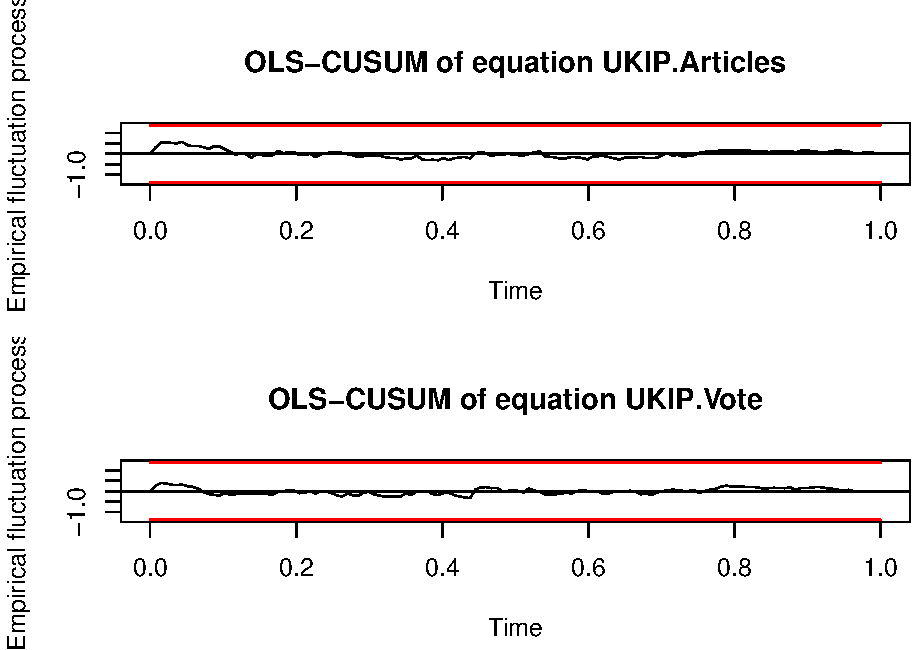
\includegraphics{ukip_media_files/figure-latex/supplementary-1.pdf}
\caption{}
\end{figure}

\pagebreak

\section{References}\label{references}

\raggedright

\hyperdef{}{ref-Achen:2006fp}{\label{ref-Achen:2006fp}}
Achen, Christopher H. (2006) ``Let's Put Garbage-Can Regressions and
Garbage-Can Probits Where They Belong.'' \emph{Conflict Management and
Peace Science} 22:327--339.

\hyperdef{}{ref-ux5felectionux5f2005}{\label{ref-ux5felectionux5f2005}}
Anon. (2005) ``Election 2005: UKIP and Greens fail to make gains.''
\emph{The Guardian}.

\hyperdef{}{ref-Baum:2012je}{\label{ref-Baum:2012je}}
Baum, Matthew A. (2012) ``The Iraq Coalition of the Willing and
(Politically) Able: Party Systems, the Press, and Public Influence on
Foreign Policy.'' \emph{American Journal of Political Science}
57:442--458.

\hyperdef{}{ref-BBC:R6UMvIKM}{\label{ref-BBC:R6UMvIKM}}
BBC. (2015) ``Appendix I Party Coverage 2015.''
\url{http://downloads.bbc.co.uk/bbctrust/assets/files/pdf/our_work/election_guidelines/2015/draft_election_guidelines_appendix.pdf}.

\hyperdef{}{ref-beckux5fsocialux5f2002}{\label{ref-beckux5fsocialux5f2002}}
Beck, Paul Allen, Russell J. Dalton, Steven Greene, and Robert
Huckfeldt. (2002) ``The Social Calculus of Voting: Interpersonal, Media,
and Organizational Influences on Presidential Choices.'' \emph{The
American Political Science Review} 96:57--73.
\url{http://www.jstor.org/stable/3117810} (Accessed October 26, 2015).

\hyperdef{}{ref-Benson:2009kb}{\label{ref-Benson:2009kb}}
Benson, Rodney. (2009) ``What makes news more multiperspectival? A field
analysis.'' \emph{Poetics} 37:402--418.
\url{http://linkinghub.elsevier.com/retrieve/pii/S0304422X09000412}.

\hyperdef{}{ref-Boomgaarden:2007ia}{\label{ref-Boomgaarden:2007ia}}
Boomgaarden, Hajo G, and Rens Vliegenthart. (2007) ``Explaining the rise
of anti-immigrant parties: The role of news media content.''
\emph{Electoral Studies} 26:404--417.

\hyperdef{}{ref-Boomgaarden:2009ke}{\label{ref-Boomgaarden:2009ke}}
Boomgaarden, Hajo G, and Rens Vliegenthart. (2009) ``How news content
influences anti-immigration attitudes: Germany, 19932005.''
\emph{European Journal of Political Research} 48:516--542.

\hyperdef{}{ref-Bos:2011iy}{\label{ref-Bos:2011iy}}
Bos, Linda, Wouter van der Brug, and Claes de Vreese. (2011) ``How the
Media Shape Perceptions of Right-Wing Populist Leaders.''
\emph{Political Communication} 28:182--206.

\hyperdef{}{ref-brandt2007multiple}{\label{ref-brandt2007multiple}}
Brandt, Patrick T, and John Taylor Williams. 2007. \emph{Multiple time
series models}. London: Sage.

\hyperdef{}{ref-daltonux5fpartisanux5f1998}{\label{ref-daltonux5fpartisanux5f1998}}
Dalton, Russell J., Paul A. Beck, and Robert Huckfeldt. (1998)
``Partisan Cues and the Media: Information Flows in the 1992
Presidential Election.'' \emph{The American Political Science Review}
92:111--126. \url{http://www.jstor.org/stable/2585932} (Accessed October
3, 2015).

\hyperdef{}{ref-Duverger:1972wk}{\label{ref-Duverger:1972wk}}
Duverger, Maurice. (1972) ``Factors in a two-party and multiparty
system.'' \emph{Party politics and pressure groups}. New York
\url{http://scholar.google.com/scholar?q=related:rSp_PasTzcEJ:scholar.google.com/\&hl=en\&num=20\&as_sdt=0,5}.

\hyperdef{}{ref-fordux5fstrategicux5f2012}{\label{ref-fordux5fstrategicux5f2012}}
Ford, Robert, Matthew J. Goodwin, and David Cutts. (2012) ``Strategic
Eurosceptics and polite xenophobes: Support for the United Kingdom
Independence Party (UKIP) in the 2009 European Parliament elections.''
\emph{European Journal of Political Research} 51:204--234.
\url{http://onlinelibrary.wiley.com/doi/10.1111/j.1475-6765.2011.01994.x/abstract}
(Accessed November 16, 2015).

\hyperdef{}{ref-Gerring:2015ub}{\label{ref-Gerring:2015ub}}
Gerring, John. (2015) ``The relevance of relevance.'' In: Gerry Stoker,
Guy B Peters, and Jon Pierre (eds) \emph{The relevance of political
science}. London: Palgrave Macmillan
\url{http://blogs.bu.edu/jgerring/files/2014/11/Chapter-2.pdf}.

\hyperdef{}{ref-goodmanux5fdoesux5f2013}{\label{ref-goodmanux5fdoesux5f2013}}
Goodman, Paul. (2013) ``Does Mr Farage want to destroy the
Conservatives, or join them?; By urging ministers to accept Syrian
refugees, Ukip's leader has played a very canny game.'' \emph{The Daily
Telegraph}.

\hyperdef{}{ref-Goodwin:03LtHfhh}{\label{ref-Goodwin:03LtHfhh}}
Goodwin, Matthew, and Robert Ford. (2013) ``Just how much media coverage
does UKIP get?'' \emph{New Statesman}.
\url{http://www.newstatesman.com/politics/2013/11/just-how-much-media-coverage-does-ukip-get}.

\hyperdef{}{ref-hopmannux5feffectsux5f2010}{\label{ref-hopmannux5feffectsux5f2010}}
Hopmann, David Nicolas, Rens Vliegenthart, Claes De Vreese, and Erik
Albæk. (2010) ``Effects of Election News Coverage: How Visibility and
Tone Influence Party Choice.'' \emph{Political Communication}
27:389--405. \url{http://dx.doi.org/10.1080/10584609.2010.516798}
(Accessed October 10, 2015).

\hyperdef{}{ref-IpsosMORI:gm2fXYNK}{\label{ref-IpsosMORI:gm2fXYNK}}
Ipsos-MORI. (n.d.) ``Voting Intention in Great Britain: Recent Trends.''
\url{https://www.ipsos-mori.com/researchpublications/researcharchive/poll.aspx?oItemId=107\&view=wide}.

\hyperdef{}{ref-koopmansux5friseux5f2009}{\label{ref-koopmansux5friseux5f2009}}
Koopmans, Ruud, and Jasper Muis. (2009) ``The rise of right-wing
populist Pim Fortuyn in the Netherlands: A discursive opportunity
approach.'' \emph{European Journal of Political Research} 48:642--664.
\url{http://onlinelibrary.wiley.com/doi/10.1111/j.1475-6765.2009.00846.x/abstract}
(Accessed October 10, 2015).

\hyperdef{}{ref-Kumlin:2001iq}{\label{ref-Kumlin:2001iq}}
Kumlin, Staffan. (2001) ``IdeologyDriven opinion formation in Europe:
The case of attitudes towards the third sector in Sweden.''
\emph{European Journal of Political Research} 39:487--518.
\url{http://onlinelibrary.wiley.com.libproxy.temple.edu/doi/10.1111/1475-6765.00585/abstract}.

\hyperdef{}{ref-martinux5fimmigrationux5f2013}{\label{ref-martinux5fimmigrationux5f2013}}
Martin, Iain. (2013) ``Immigration from Romania and Bulgaria set to give
Nigel Farage and Ukip a boost.'' \emph{The Telegraph}.
\url{http://blogs.telegraph.co.uk/news/iainmartin1/100252078/immigration-from-romania-and-bulgaria-set-to-give-nigel-farage-and-ukip-a-boost/}.

\hyperdef{}{ref-morrisux5felectionux5f2005}{\label{ref-morrisux5felectionux5f2005}}
Morris, Nigel. (2005) ``Election 2005: UKIP's bubble may have burst, but
Kilroy-Silk's party also fails to take off.'' \emph{The Independent}.

\hyperdef{}{ref-murphyux5fukipux5f2015}{\label{ref-murphyux5fukipux5f2015}}
Murphy, Justin. (2015) ``Ukip don't deserve their media prominence.
Here's the proof.'' \emph{New Statesman}.
\url{http://www.newstatesman.com/politics/2015/04/ukip-dont-deserve-their-media-prominence-heres-proof}.

\hyperdef{}{ref-norrisux5fvirtuousux5f2000}{\label{ref-norrisux5fvirtuousux5f2000}}
Norris, Pippa. 2000. \emph{A Virtuous Circle: Political Communications
in Postindustrial Societies}. Cambridge, UK: Cambridge University Press
\url{http://www.cambridge.org/gb/academic/subjects/politics-international-relations/comparative-politics/virtuous-circle-political-communications-postindustrial-societies}.

\hyperdef{}{ref-oegemaux5fpersonalizationux5f2009}{\label{ref-oegemaux5fpersonalizationux5f2009}}
Oegema, Dirk, and Jan Kleinnijenhuis. (2009) ``Personalization in
political Television News: A 13-Wave Survey Study to Assess Effects of
Text and Footage.'' \emph{Communications} 25:43--60.
\url{http://www.degruyter.com/view/j/comm.2000.25.issue-1/comm.2000.25.1.43/comm.2000.25.1.43.xml}
(Accessed October 26, 2015).

\hyperdef{}{ref-Ofcom:2015tt}{\label{ref-Ofcom:2015tt}}
Ofcom. (2015) ``Ofcom list of major parties.''
\url{http://stakeholders.ofcom.org.uk/binaries/broadcast/guidance/major-parties.pdf}.

\hyperdef{}{ref-paletzux5fpoliticalux5f1996}{\label{ref-paletzux5fpoliticalux5f1996}}
Paletz, David. 1996. \emph{Political communication research: Vol. 2.
Approaches, studies, assessments}. Norwood, NJ: Ablex.

\hyperdef{}{ref-pauwelsux5freassessingux5f2010}{\label{ref-pauwelsux5freassessingux5f2010}}
Pauwels, Teun. (2010) ``Reassessing conceptualization, data and
causality: A critique of Boomgaarden and Vliegenthart's study on the
relationship between media and the rise of anti-immigrant parties.''
\emph{Electoral Studies} 29:269--275.
\url{http://www.sciencedirect.com/science/article/pii/S0261379410000120}
(Accessed October 10, 2015).

\hyperdef{}{ref-rooduijnux5fmesmerisingux5f2014}{\label{ref-rooduijnux5fmesmerisingux5f2014}}
Rooduijn, Matthijs. (2014) ``The Mesmerising Message: The Diffusion of
Populism in Public Debates in Western European Media.'' \emph{Political
Studies} 62:726--744.
\url{http://onlinelibrary.wiley.com/doi/10.1111/1467-9248.12074/abstract}
(Accessed October 2, 2015).

\hyperdef{}{ref-sellersux5fwinningux5f2007}{\label{ref-sellersux5fwinningux5f2007}}
Sellers, Patrick J., and Brian F. Schaffner. (2007) ``Winning Coverage
in the U.S. Senate.'' \emph{Political Communication} 24:377--391.
\url{http://dx.doi.org/10.1080/10584600701641516} (Accessed October 11,
2015).

\hyperdef{}{ref-semetkoux5fgermanysux5f1994}{\label{ref-semetkoux5fgermanysux5f1994}}
Semetko, Holli A, and Klaus Schoenbach. 1994. \emph{Germany's Unity
Election: Voters and the Media}. Cresskill: Hampton Press.

\hyperdef{}{ref-Sheafer:2009hi}{\label{ref-Sheafer:2009hi}}
Sheafer, Tamir, and Gadi Wolfsfeld. (2009) ``Party Systems and
Oppositional Voices in the News Media A Study of the Contest over
Political Waves in the United States and Israel.'' \emph{The
International Journal of Press/Politics} 14:146--165.
\url{http://hij.sagepub.com/cgi/doi/10.1177/1940161209333089}.

\hyperdef{}{ref-Soussi:vy}{\label{ref-Soussi:vy}}
Soussi, Alasdair. (2014) ``Did British media help the UKIP win EU
poll?''
\url{http://www.aljazeera.com/indepth/features/2014/06/did-british-media-help-ukip-win-eu-poll-20146313346918679.html}.

\hyperdef{}{ref-Stevenson:wo}{\label{ref-Stevenson:wo}}
Stevenson, Alex. (2014) ``Caroline Lucas points finger at media's Farage
obsession.''
\url{http://www.politics.co.uk/news/2014/05/29/ukip-victory-caroline-lucas-points-finger-at-media-s-farage}.

\hyperdef{}{ref-Stromback:2006ht}{\label{ref-Stromback:2006ht}}
Strömbäck, Jesper, and Daniela V Dimitrova. (2006) ``Political and Media
Systems Matter A Comparison of Election News Coverage in Sweden and the
United States.'' \emph{The International Journal of Press/Politics}
11:131--147.
\url{http://hij.sagepub.com.libproxy.temple.edu/content/11/4/131.abstract}.

\hyperdef{}{ref-Sweeney:wp}{\label{ref-Sweeney:wp}}
Sweeney, Mark. (2015) ``BBC prepares to boost Ukip coverage as it ranks
it a larger party in election.''
\url{http://www.theguardian.com/media/2015/jan/15/bbc-prepares-to-boost-ukip-coverage-as-it-ranks-it-a-larger-party-in-election}.

\hyperdef{}{ref-treschux5fpoliticiansux5f2009}{\label{ref-treschux5fpoliticiansux5f2009}}
Tresch, Anke. (2009) ``Politicians in the Media: Determinants of
Legislators' Presence and Prominence in Swiss Newspapers.'' \emph{The
International Journal of Press/Politics} 14:67--90.
\url{http://hij.sagepub.com/content/14/1/67} (Accessed October 11,
2015).

\hyperdef{}{ref-Vliegenthart:2014di}{\label{ref-Vliegenthart:2014di}}
Vliegenthart, Rens. (2014) ``Moving up. Applying aggregate level time
series analysis in the study of media coverage.'' \emph{Quality \&
Quantity} 48:2427--2445.

\hyperdef{}{ref-vliegenthartux5fwhyux5f2010}{\label{ref-vliegenthartux5fwhyux5f2010}}
Vliegenthart, Rens, and Hajo G. Boomgaarden. (2010) ``Why the media
matter after all: A response to Pauwels.'' \emph{Electoral Studies}
29:719--723.
\url{http://www.sciencedirect.com/science/article/pii/S0261379410000855}
(Accessed October 11, 2015).

\hyperdef{}{ref-vliegenthartux5fanti-immigrantux5f2012}{\label{ref-vliegenthartux5fanti-immigrantux5f2012}}
Vliegenthart, Rens, Hajo G. Boomgaarden, and Joost Van Spanje. (2012)
``Anti-Immigrant Party Support and Media Visibility: A Cross-Party,
Over-Time Perspective.'' \emph{Journal of Elections, Public Opinion and
Parties} 22:315--358.
\url{http://dx.doi.org/10.1080/17457289.2012.693933} (Accessed October
10, 2015).

\hyperdef{}{ref-wainwrightux5frotherhamux5f2012}{\label{ref-wainwrightux5frotherhamux5f2012}}
Wainwright, Martin. (2012) ``Rotherham byelection brings relief for
Labour as Ukip celebrates second place.'' \emph{The Guardian}.
\url{http://www.theguardian.com/politics/2012/nov/30/rotherham-byelection-labour-ukip}.

\hyperdef{}{ref-walgraveux5fmakingux5f2004}{\label{ref-walgraveux5fmakingux5f2004}}
Walgrave, Stefaan, and Knut De Swert. (2004) ``The Making of the (Issues
of the) Vlaams Blok.'' \emph{Political Communication} 21:479--500.
\url{http://dx.doi.org/10.1080/10584600490522743} (Accessed October 10,
2015).

\hyperdef{}{ref-wattux5feuropeanux5f2009}{\label{ref-wattux5feuropeanux5f2009}}
Watt, Nicholas, and Matthew Taylor. (2009) ``European Elections: Ukip:
Eurosceptics claim second place is political earthquake.'' \emph{The
Guardian}.

\hyperdef{}{ref-Whitaker:2011gi}{\label{ref-Whitaker:2011gi}}
Whitaker, Richard, and Philip Lynch. (2011) ``Explaining Support for the
UK Independence Party at the 2009 European Parliament Elections.''
\emph{Journal of Elections, Public Opinion \& Parties} 21:359--379.
\url{http://www.tandfonline.com/doi/abs/10.1080/17457289.2011.588439}.

\hyperdef{}{ref-whiteux5fukipux5f2006}{\label{ref-whiteux5fukipux5f2006}}
White, Michael, and Nicholas Watt. (2006) ``Ukip threatens to sue over
Cameron's 'racist' remark.'' \emph{The Guardian}.
\url{http://www.theguardian.com/uk/2006/apr/05/otherparties.politics}
(Accessed November 16, 2015).

\hyperdef{}{ref-winnettux5ftoryux5f2008}{\label{ref-winnettux5ftoryux5f2008}}
Winnett, Robert, and Rosa Prince. (2008) ``Tory defector becomes Ukip's
first MP.'' \emph{The Daily Telegraph}.

\hyperdef{}{ref-Wintour:vf}{\label{ref-Wintour:vf}}
Wintour, Patrick. (2015) ``Ofcom deals blow to Greens election debate
hopes but boosts Ukips.''
\url{http://www.theguardian.com/politics/2015/jan/08/ofcom-blow-green-party-election-debate-boost-ukips}.

\end{document}
